\documentclass{article}

\usepackage{booktabs}
\usepackage{tabularx}
\usepackage{hyperref}
\usepackage{color, colortbl}
\usepackage{graphicx,array}
\usepackage{enumitem}
\usepackage{multirow}
\hypersetup{
    colorlinks=true,       % false: boxed links; true: colored links
    linkcolor=red,          % color of internal links (change box color with linkbordercolor)
    citecolor=green,        % color of links to bibliography
    filecolor=magenta,      % color of file links
    urlcolor=cyan           % color of external links
}

\title{Hazard Analysis\\\progname}

\author{\authname}

\date{}

%% Comments

\usepackage{color}

\newif\ifcomments\commentstrue %displays comments
%\newif\ifcomments\commentsfalse %so that comments do not display

\ifcomments
\newcommand{\authornote}[3]{\textcolor{#1}{[#3 ---#2]}}
\newcommand{\todo}[1]{\textcolor{red}{[TODO: #1]}}
\else
\newcommand{\authornote}[3]{}
\newcommand{\todo}[1]{}
\fi

\newcommand{\wss}[1]{\authornote{blue}{SS}{#1}} 
\newcommand{\plt}[1]{\authornote{magenta}{TPLT}{#1}} %For explanation of the template
\newcommand{\an}[1]{\authornote{cyan}{Author}{#1}}

%% Common Parts

\newcommand{\progname}{ProgName} % PUT YOUR PROGRAM NAME HERE
\newcommand{\authname}{Team \#, Team Name
\\ Student 1 name and macid
\\ Student 2 name and macid
\\ Student 3 name and macid
\\ Student 4 name and macid} % AUTHOR NAMES                  

\usepackage{hyperref}
    \hypersetup{colorlinks=true, linkcolor=blue, citecolor=blue, filecolor=blue,
                urlcolor=blue, unicode=false}
    \urlstyle{same}
                                


\begin{document}

\maketitle
\thispagestyle{empty}

~\newpage

\pagenumbering{roman}

\begin{table}[hp]
\caption{Revision History} \label{TblRevisionHistory}
\begin{tabularx}{\textwidth}{llX}
\toprule
\textbf{Date} & \textbf{Developer(s)} & \textbf{Change}\\
\midrule
Date1 & Name(s) & Description of changes\\
Date2 & Name(s) & Description of changes\\
... & ... & ...\\
\bottomrule
\end{tabularx}
\end{table}

~\newpage

\tableofcontents

~\newpage

\pagenumbering{arabic}

\wss{You are free to modify this template.}

\section{Introduction}

\wss{You can include your definition of what a hazard is here.}

\section{Scope and Purpose of Hazard Analysis}

\section{System Boundaries and Components}
The system consists of several components that make up the entire system

	\subsection{Battery/Power Management system}
		This component facilitates stepping down/up the source voltage from the battery to the necessary values required by different parts of the device. Moreover, it consists of a 										charge protection circuit for battery protection (Over-voltage and Discharge). Finally present is a battery level indicator that will generate an alert should the battery life fall below a certain threshold.  

	\subsection{Sensor Array system}
		This component represents all the various sensors that will be used to collect the state information about the user. Also consists of various filters to facilitate smooth and accurate data collection.

	\subsection{Prompt generation system}
		This component handles  all prompt generation, from the detection of when a prompt occurs, to its specific creation and finally its display on the screen.
	
	\subsection{Display System}
		This system manages all functionality of the device's display, such as prompt display, showing basic user feedback such as date, time, temperature, etc. 
	
	\subsection{Data Storage system} 
		This system handles all logging and storage of data collected by both the sensor array and the prompt generator. Data is stored along with an indication of which system it came from and all prompts will be 				stored with the data and time of entry.

	\subsection{Device Manager}
		This system handles all connection and communication between the device and the host software.
	
	\subsection{Error Handler - Hardware}
		This component constantly checks the states of every system present and ensures that if any of them fail or return an error, an alert is generated. Moreover the system will also try to fix the problem 					wherever possible.

	\subsection{Error Handler - Software}
		This component monitors the state of the host software and will attempt to solve any errors that arise and will alert the user should the attempts fail.

	\subsection{Host Software}
		This system is the primary interface for the researchers to analyze the data collected by the device. It consists of several features that allows the researcher to set different 					
		thresholds for activity tracking, calibrate all the sensors, update and create new records for participants, and finally interact with the data stored on the device.

	\subsection{Calibration}
		This system allows researchers to calibrate the sensors on the device , set and modify the different thresholds for activity tracking and create new prompts. 

	\subsection{Records}
		This system stores all information about users present in the study. Moreover it provides functionality for researchers to create new records for new users.

	\subsection{Data View}
		This is where all data stored on the device can be viewed/ analyzed by the researchers in a graphical manner. The system also contains some functionality for data sorting/parsing and statistical analysis.
	
	\subsection{System Boundary Diagram}
		\begin{figure}
			\begin{center}
				 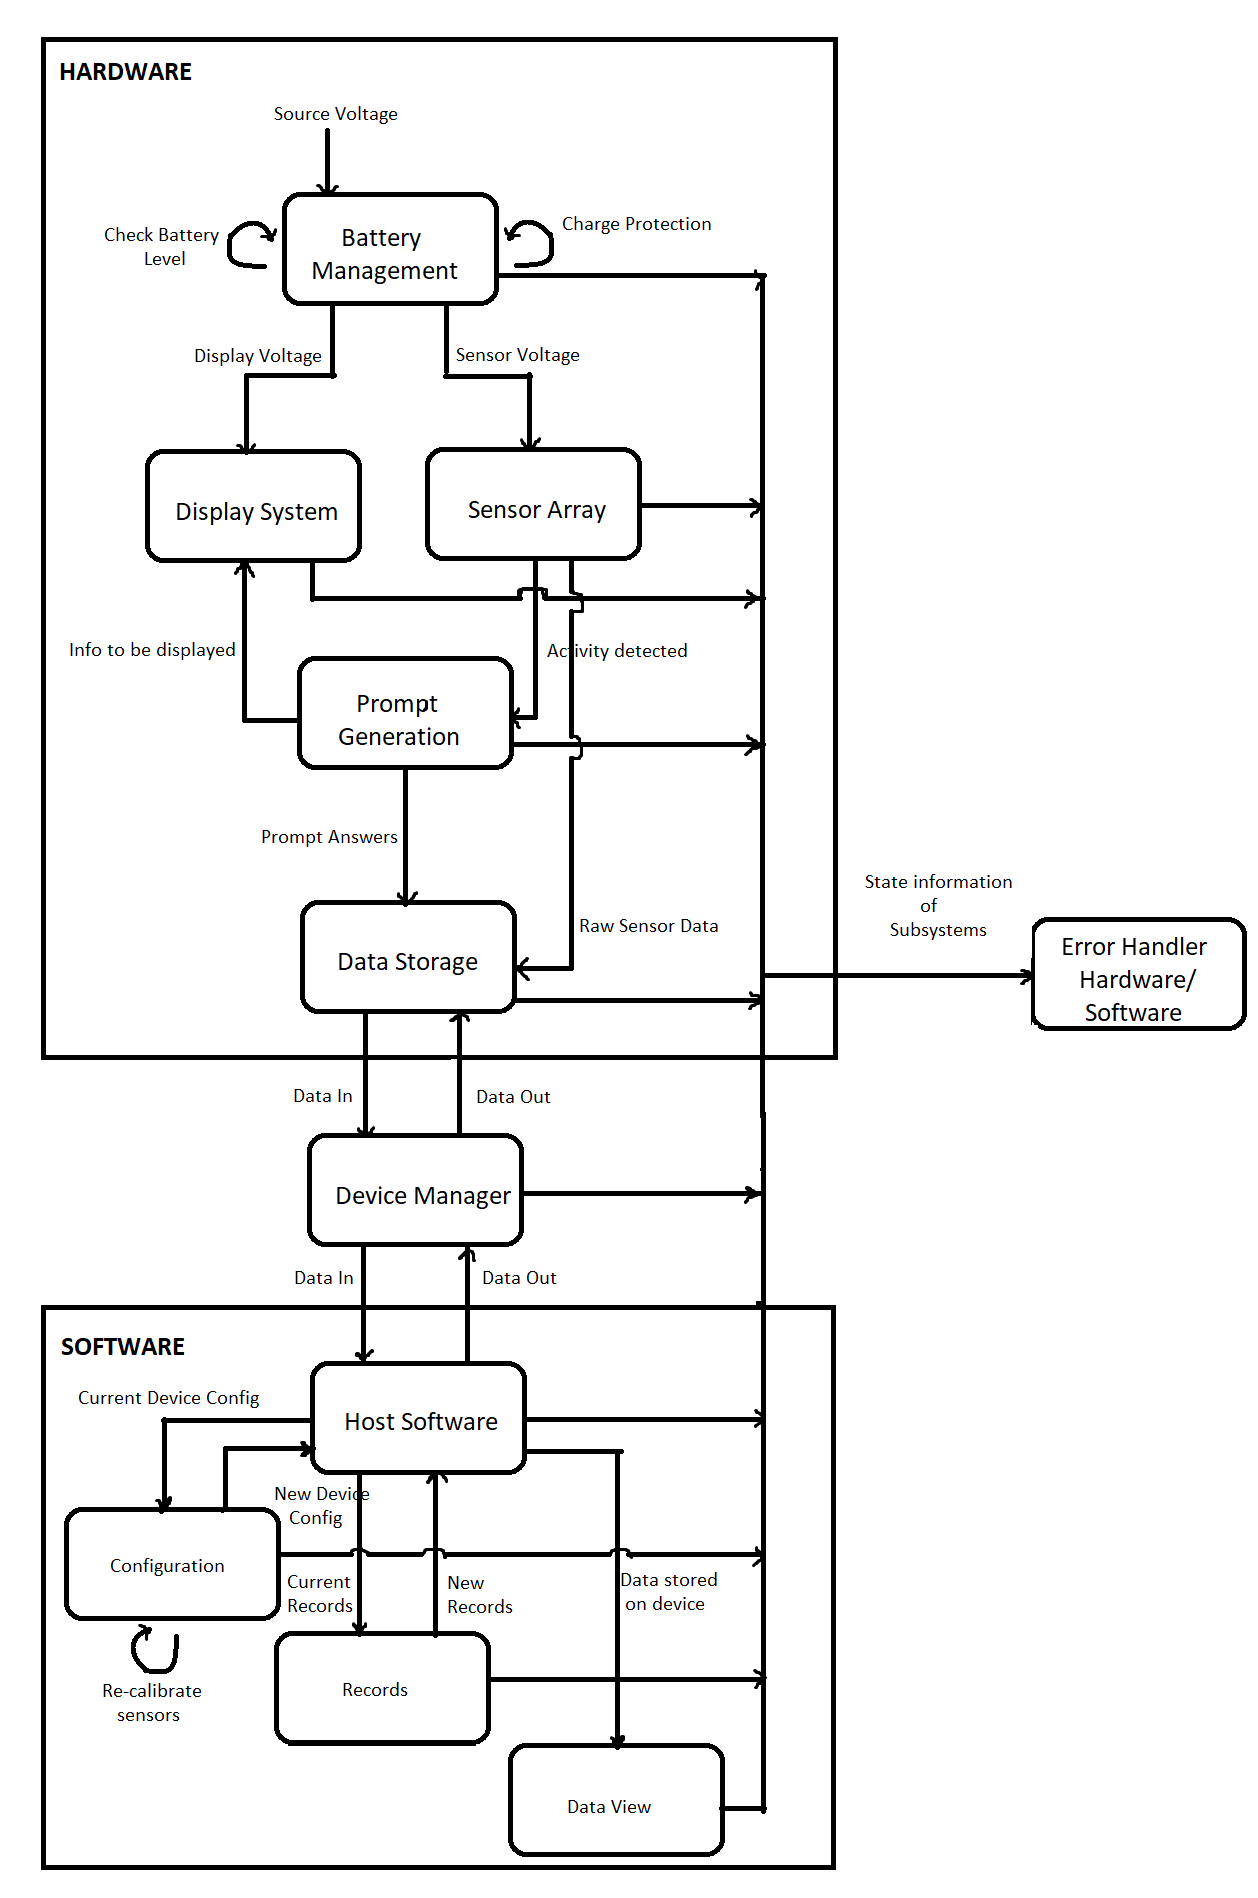
\includegraphics[width=1.0\textwidth]{SystemBoundaryDiagram}
				\caption{System Boundary Diagram}
				\label{Fig_SBD} 
			\end{center}
		\end{figure}	
\pagebreak
	 
\section{Critical Assumptions }

\wss{These assumptions that are made about the software or system.  You should
minimize the number of assumptions that remove potential hazards.  For instance,
you could assume a part will never fail, but it is generally better to include
this potential failure mode.}

\section{Failure Mode and Effect Analysis}
\begin{tabular}{|m{6em}|m{5em}|m{5em}|m{5em}|m{5em}|m{9em}|}
\hline
    
    \textbf{Design Component} & \textbf{Failure Modes}   & \textbf{Causes of Failure}   & \textbf{Effects of Failure}   & \textbf{Detection}   & \textbf{Recommended Action}\tabularnewline\hline
 %%%%%%%%%%%%%%%%%%%%%%%%%%%%%%%%%%%%%%%%%%%%%%%%%%%%%%%%%%%%%%%%%%%%%%%%%%%%%%%%%%%%%%%%%%%%%%%%%%%%%%%

          & Display not working & 
		    \begin{minipage}[t]{\linewidth}
		        \begin{itemize}[nosep, wide=0pt, leftmargin=*, after=\strut]
		            \item Improper circuit connection
		            \item Battery Level too low
		            \item Code malfunction
			    \item Physical damage to display
		        \end{itemize}
		    \end{minipage}

          & 	      \begin{itemize}[nosep, wide=0pt, leftmargin=*, after=\strut]
		            \item Users cannot answer prompts.
		            \item Users cannot view any information on the display
		        \end{itemize}

	  & Display system returns an error code. Display Led is OFF
          & \begin{itemize}[nosep, wide=0pt, leftmargin=*, after=\strut]
		            \item Users cannot answer prompts.
		            \item Users cannot view any information on the display
			    \item Check wiring and run a diagnostic on the display system
			    \item Replace faulty hardware 
		        \end{itemize}
		  \tabularnewline\cline{2-6}

 %%%%%%%%%%%%%%%%%%%%%%%%%%%%%%%%%%%%%%%%%%%%%%%%%%%%%%%%%%%%%%%%%%%%%%%%%%%%%%%%%%%%%%%%%%%%%%%%%%%%%%%

    \multirow{-8}{*}{\centering\rotatebox[origin=c]{90}{Display System}}
                             
	 & Incorrect information displayed      
	 & \begin{minipage}[t]{\linewidth}
           	 \begin{itemize}[nosep, wide=0pt, leftmargin=*, after=\strut]
		            \item Display Driver faulty
		            \item Improper interaction between Display system and Prompt generation
       		 \end{itemize}
             \end{minipage}                             

	& Users face unexpected outputs causing imporper use of device                                                                
        & Display system returns an error code.

        & \begin{minipage}[t]{\linewidth}
              \begin{itemize}[nosep, wide=0pt, leftmargin=*, after=\strut]
	            \item Let Error Handler try to solve issue.
	            \item Perform a manual overview of code.
		    \item Perform a system reboot.
               \end{itemize}
            \end{minipage}  \tabularnewline\cline{1-6}
\end{tabular}%\vspace{3mm}
 %%%%%%%%%%%%%%%%%%%%%%%%%%%%%%%%%%%%%%%%%%%%%%%%%%%%%%%%%%%%%%%%%%%%%%%%%%%%%%%%%%%%%%%%%%%%%%%%%%%%%%%


\begin{tabular}{|m{6em}|m{5em}|m{5em}|m{5em}|m{5em}|m{9em}|}
    

 %%%%%%%%%%%%%%%%%%%%%%%%%%%%%%%%%%%%%%%%%%%%%%%%%%%%%%%%%%%%%%%%%%%%%%%%%%%%%%%%%%%%%%%%%%%%%%%%%%%%%%%

	  \hline
          & Prompt not generated & 
		    \begin{minipage}[t]{\linewidth}
		        \begin{itemize}[nosep, wide=0pt, leftmargin=*, after=\strut]
		            \item Prompt generation code faulty
		            \item System stuck in an idle state where no activity is detected.
		        \end{itemize}
		    \end{minipage}

          & 	      
			\begin{itemize}[nosep, wide=0pt, leftmargin=*, after=\strut]
		            \item Display system will not produce an output.
			    \item Users will be unable to provide feedback regarding activity
		        \end{itemize}

	  & Prompt Generation system returns an error code.
          & Let Error Handle try to solve the issue  \tabularnewline\cline{2-6}

 %%%%%%%%%%%%%%%%%%%%%%%%%%%%%%%%%%%%%%%%%%%%%%%%%%%%%%%%%%%%%%%%%%%%%%%%%%%%%%%%%%%%%%%%%%%%%%%%%%%%%%%

    \multirow{-8}{*}{\centering\rotatebox[origin=c]{90}{Prompt Generation System}}
                             
	 & Incorrect Prompt Generated
	 & \begin{minipage}[t]{\linewidth}
           	 \begin{itemize}[nosep, wide=0pt, leftmargin=*, after=\strut]
		            \item Prompt generation code faulty
		            \item Improper interaction between Prompt generation and Sensor Array
       		 \end{itemize}
             \end{minipage}                             

	& Prompt generated produces unexpected outputs causing imporper use of device                                                                
        & Prompt Generation system returns an error code. Test prompt produces unexpeted outputs

        & \begin{minipage}[t]{\linewidth}
              \begin{itemize}[nosep, wide=0pt, leftmargin=*, after=\strut]
	            \item Let Error Handler try to solve issue.
	            \item Check System Array State
		    \item Perform a system reboot.
               \end{itemize}
            \end{minipage}  \tabularnewline\cline{1-6}
\end{tabular}%\vspace{3mm}
 %%%%%%%%%%%%%%%%%%%%%%%%%%%%%%%%%%%%%%%%%%%%%%%%%%%%%%%%%%%%%%%%%%%%%%%%%%%%%%%%%%%%%%%%%%%%%%%%%%%%%%%









\section{Safety and Security Requirements}

\subsection{Hardware Requirements}
\textbf{HR1}: All Hardware systems will have an associated indicator LED.\\
\textbf{HR2}: Device compoments will have sufficient electrical tolerances for Current, Voltage, Temperature etc.

\subsection{Software  Requirements}
\textbf{SR1}: The Error Handler will initially try to solve all Non-Hardware issues.\\
\textbf{SR2}: System tests will be conducted before deployment of the device.\\


\subsection{Data Storage Requirements }
\textbf{DSR1}: Error reports and incorrect data will be logged into a seperate database.\\


\subsection{Data Security Requirements }










\section{Roadmap}

\wss{Which safety requirements will be implemented as part of the capstone timeline?
Which requirements will be implemented in the future?}

\section{Appendix}
 %%%%%%%%%%%%%%%%%%%%%%%%%%%%%%%%%%%%%%%%%%%%%%%%%%%%%%%%%%%%%%%%%%%%%%%%%%%%%%%%%%%%%%%%%%%%%%%%%%%%%%%
\subsection{Error Codes}
To facilitate error handling, every system will return an error code that represents the status of that system. These error codes follow the following format, BED\_ERR\_ERRORTYPE
For example BED\_ERR\_NONE represent that the system is working correctly. Some more examples of error codes are:
\begin{itemize}
\item BED\_ERR\_PARAM\_ERR		 	: Represents an error with the paramaters of the function.
\item BED\_ERR\_GENERAL			 	: Represents a generic error that hasnt been catalogued yet. 	
\item BED\_ERR\_INVALID\_DATA\_SIZE	: Represents an error related to a size mismatch in what is stored within a block of memory or variable.
\end{itemize}

 %%%%%%%%%%%%%%%%%%%%%%%%%%%%%%%%%%%%%%%%%%%%%%%%%%%%%% %%%%%%%%%%%%%%%%%%%%%%%%%%%%%%%%%%%%%%%%%%%%%%%%%































%%%%%%%%%%%%%%


\end{document}